
\documentclass{article}
\usepackage{graphicx} % Required for inserting images
\usepackage{url}

\title{KludgeCTF}
\author{Arjun Pavanje}
\date{May 2025}

\begin{document}

\maketitle
\section{Miscellaneous}
\subsection{I am not MID}
Tried the flag given in the question, and it worked :)
\section{Forensics}
\subsection{Chatty Network}
We were given a packet capture file with a suspicion that malware maybe stealing data during look ups.\newline
Analysing using Wireshark,,,
\begin{figure}[h!]
    \centering
    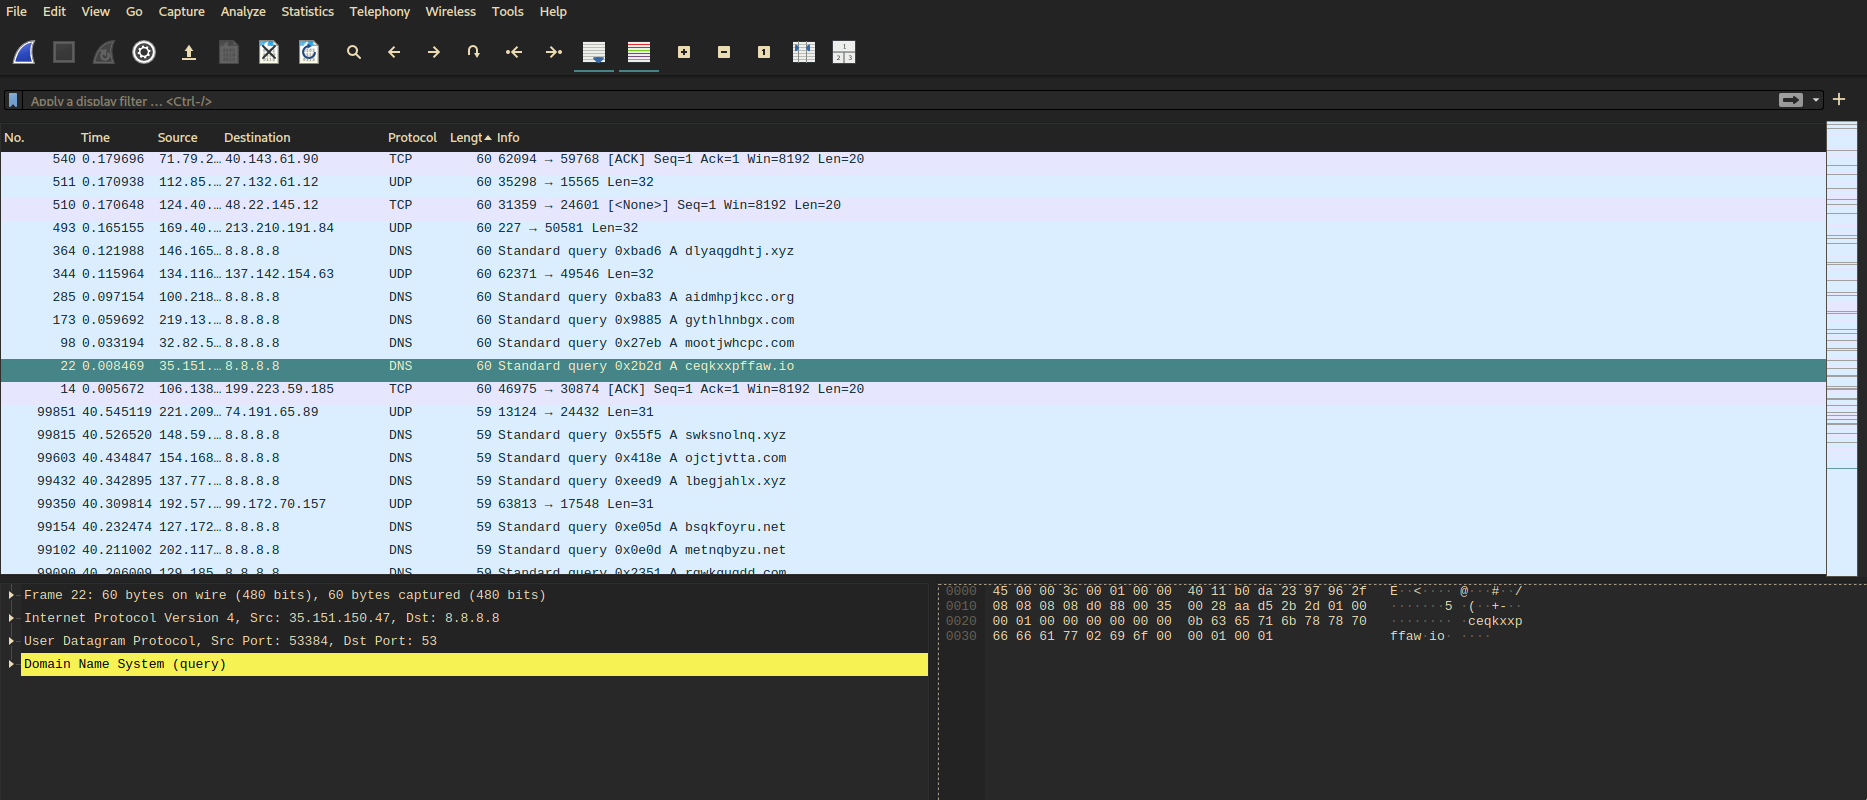
\includegraphics[width=1\linewidth]{figs/chatty_1.png}
    \label{fig:enter-label}
\end{figure}
\pagebreak
\newline Viewing all communication made using DNS protocol,
\begin{figure}[h!]
    \centering
    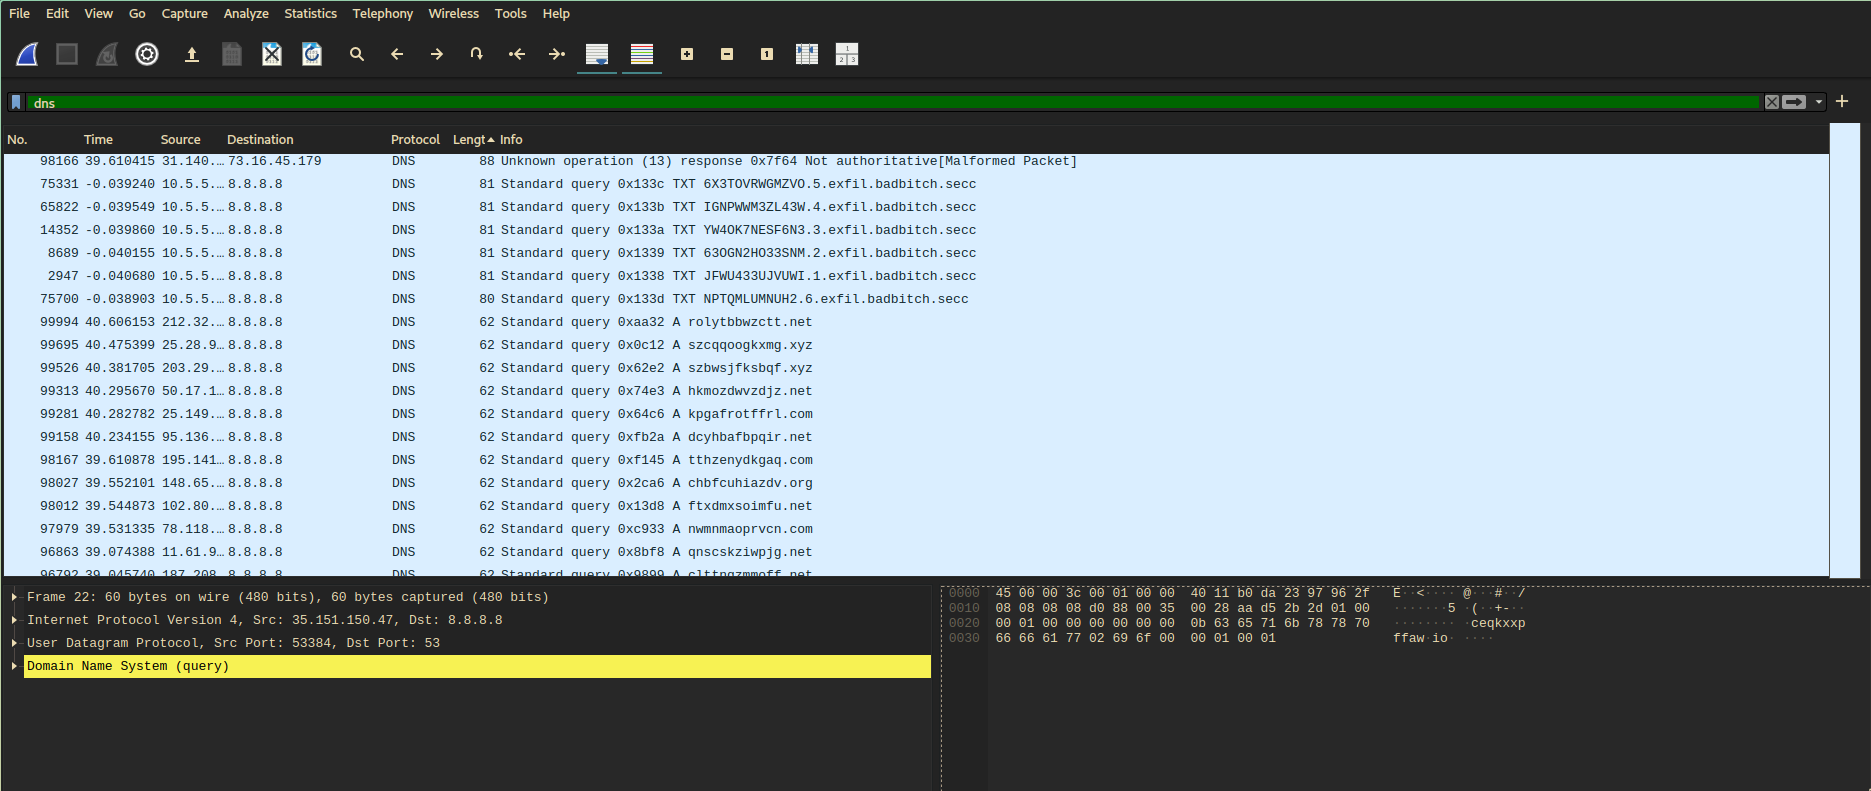
\includegraphics[width=1\linewidth]{figs/chattty_2.png}
    \label{fig:enter-label}
\end{figure}
\newline On sorting messages in descending order (size), we see 6 messages to the slightly suspicious domain $badbitch.secc$. To my observation, those 6 messages were the only ones that had the same source and destination location. So I guessed that the message may have been split into 6 parts, so I took the text from each image and tried to decode them. \newline \newline 
String obtained, $FWU433UJVUWI63OGN2HO33SNMYW4OK7NESF6\\N3IGNPWWM3ZL43W6X3TOVRWGMZVONPTQMLUMNUH2$\newline \newline 
This looked to be base-32 code, so I wrote a python code to decode it by making use of pythons $base64$ library. Python code,
\begin{verbatim}
import base64
# The three '=='s have been added as padding
encoded = "JFWU433UJVUWI63OGN2HO33SNMYW4OK7NESF6
N3IGNPWWM3ZL43W6X3TOVRWGMZVONPTQMLUMNUH2==="
decoded = base64.b32decode(encoded)
print(decoded)
\end{verbatim}
This gives us the flag, 
\begin{verbatim}
ImNotMid{n3twork1n9_i$_7h3_k3y_7o_succ35s_81tch}
\end{verbatim}
\section{Cryptography}
\subsection{Wordle}
Opened the website \url{https://core-ctf.vercel.app/},
\begin{figure}[h!]
    \centering
    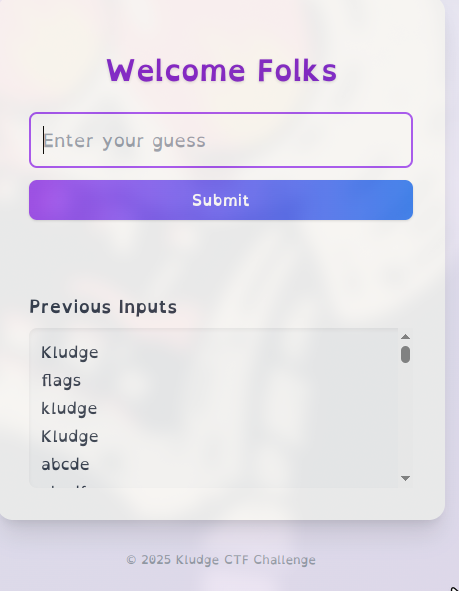
\includegraphics[width=0.5\linewidth]{figs/wordle1.png}
    \label{fig:enter-label}
\end{figure}
\pagebreak 
\newline Initially I thought that it would be a substitution or rot cypher, but after a long while of guessing words I realized that wasn't the case. I tried to find the individual number of each alphabet but realized that the number of an alphabet would be constant only for a given word size (for example the number corresponding to 'A' in PLANT and SAD would be different, but would be the same in case of 'PLANT' and 'ABCDE'). Then I abandoned such ideas and tried to check the source code by pressing $ctrl + U$, 
\begin{figure}[h!]
    \centering
    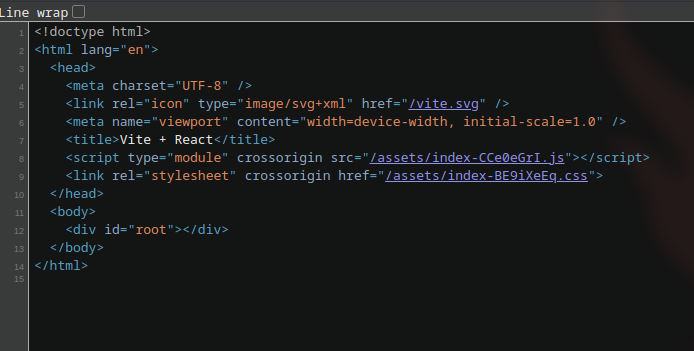
\includegraphics[width=1\linewidth]{figs/wordle2.png}
    \label{fig:enter-label}
\end{figure}
\newline Then went to \url{https://core-ctf.vercel.app/assets/index-CCe0eGrI.js} (after realizing that there was nothing on the second link), where on searching for flag (using $ctrl+F$ I got the flag 
\begin{verbatim}
imNotMid{i5\_thi5\_w3b\_0r\_crypt0}
\end{verbatim}
\begin{figure}[h!]
    \centering
    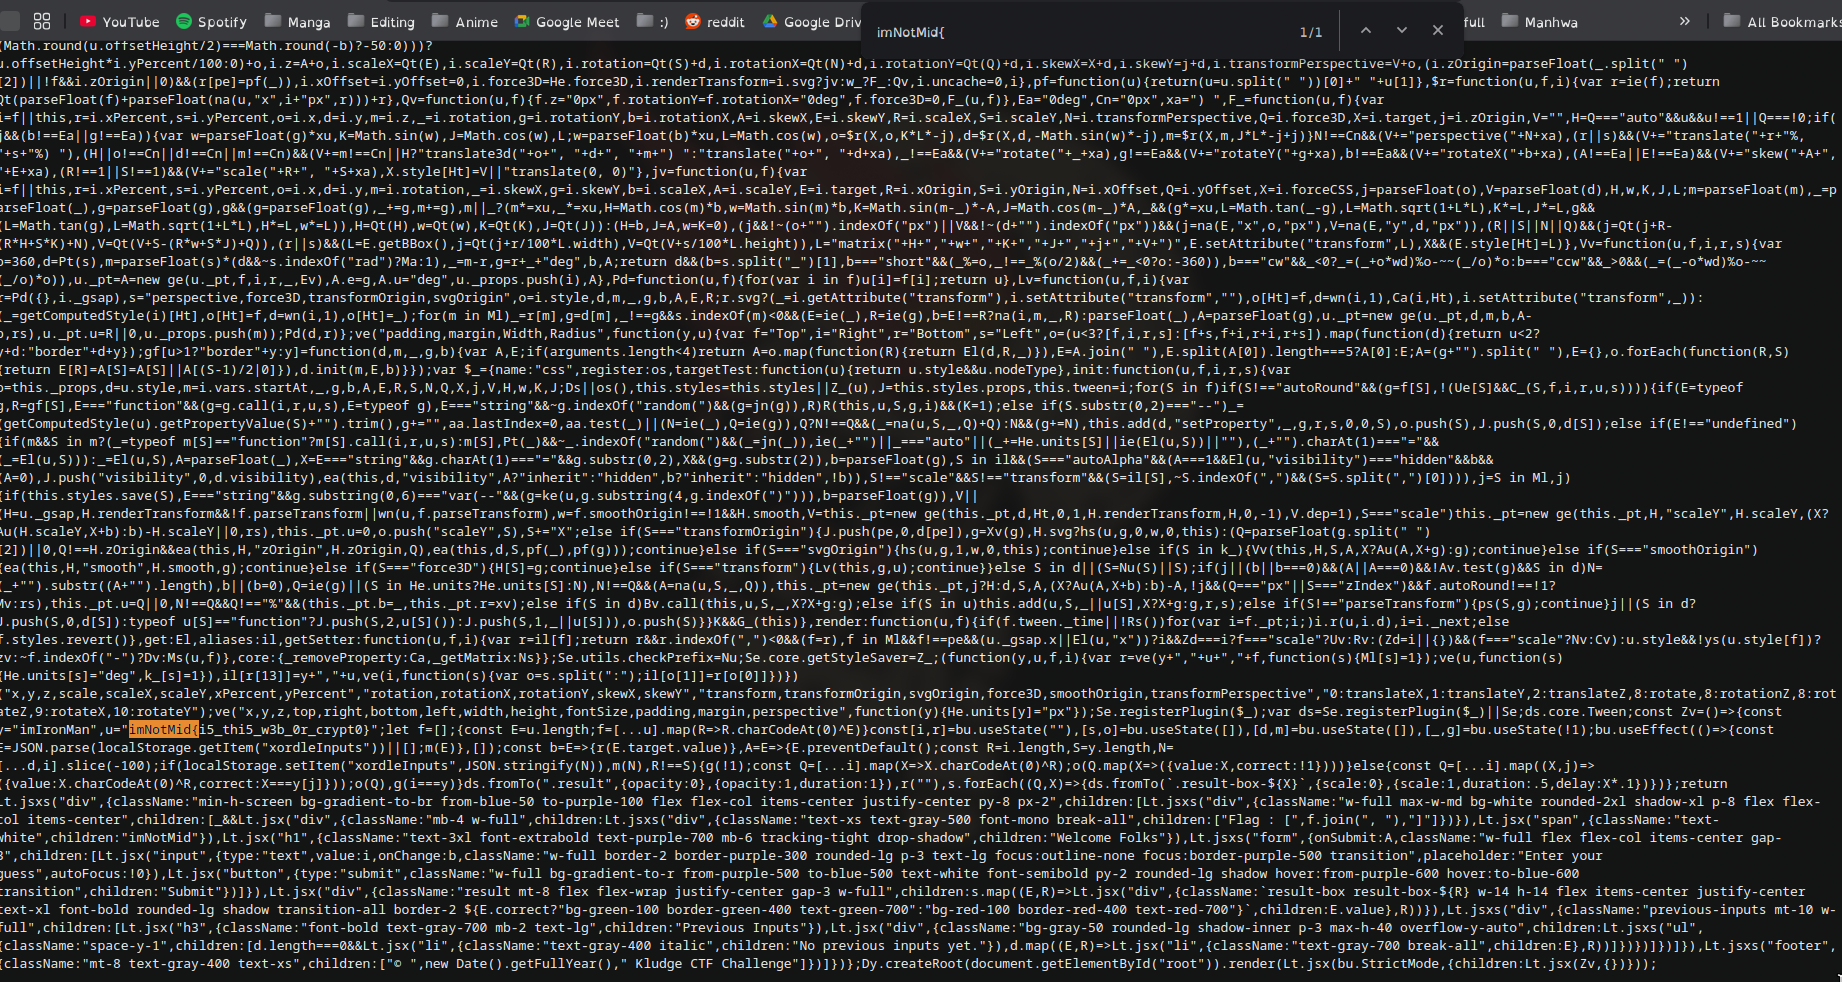
\includegraphics[width=1\linewidth]{figs/wordle3.png}
    \label{fig:enter-label}
\end{figure}
\subsection{Crypto Misstep}
Here, we are given two values of $N$ used in RSA and the standard $e = 65537$ and the cypher text. We are required to obtain the plaintext flag. Usually, it would be extremely difficult to obtain the private key, (which is given by the relation $ e*d\equiv 1 mod\varphi(n)$, whre $\varphi$ is Euler Totient function) due $N$ being an extremely large prime number (hence it is extremely difficult to calculate two prime numbers $p$, $q$ which satisfy $p\ast q = N$ ($\varphi(N)$ is given be $(p-1)(q-1)$). \newline \newline
In this case, we have two $N$ values $(N_1, N_2)$ so if they have a GCD we have found $p$, $q$ for $N_1$ and $N_2$, using which we can calculate Euler Totient function, using which we can calculate private key $d$. \newline \newline 
Python code,
\begin{figure}[h!]
    \centering
    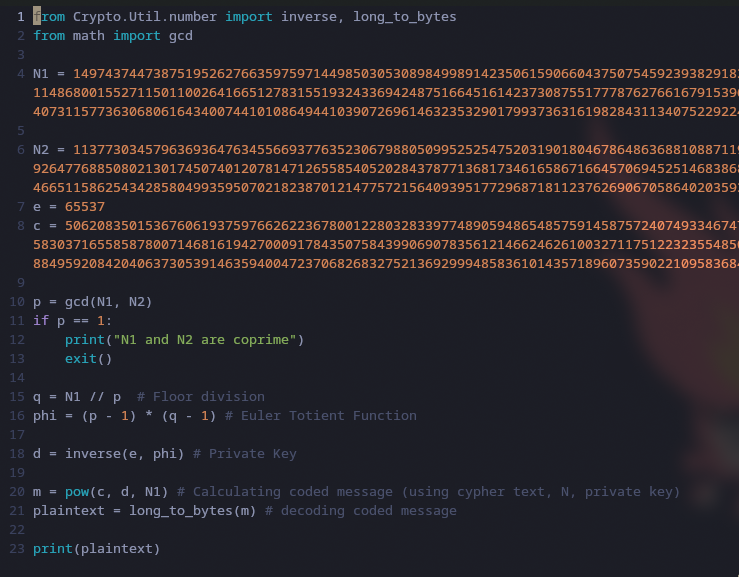
\includegraphics[width=1\linewidth]{figs/rsa.png}
    \label{fig:enter-label}
\end{figure}
\pagebreak
\newline On running the code we get the flag, 
\begin{verbatim}
ImNotMid{r54_!s_n0t_50_c00l_4nym0r3_n1994}
\end{verbatim}
\section{Reverse Engineering}
\subsection{JJK}
We are given only a binary executable, so on running it we get, 
\begin{figure}[h!]
    \centering
    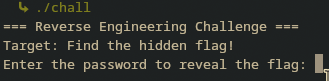
\includegraphics[width=0.6\linewidth]{figs/jjk1.png}
    \label{fig:enter-label}
\end{figure}
\newline Also on running the command \begin{verbatim}strings chall > jjk.txt \end{verbatim} we can observe a few lines of interest, 
\begin{figure}[h!]
    \centering
    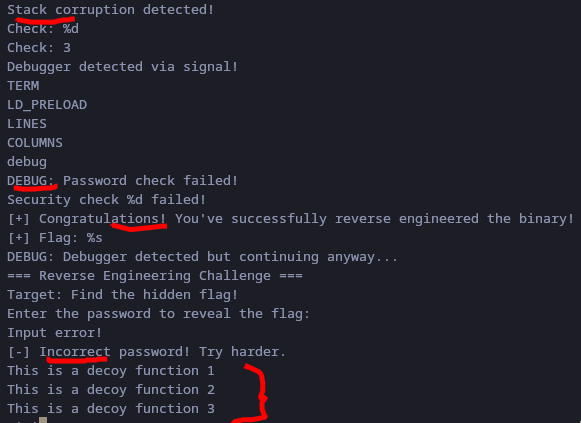
\includegraphics[width=1\linewidth]{figs/jjk2.png}
    \label{fig:enter-label}
\end{figure}
\pagebreak
\newline So we can infer that we will obtaiin the flag upon entering the right password. Since we are given nothing else, we must obtain the passphrase from the binary executable. Firstly, I disassembled the binary executable into assembly code using the command, 
\begin{verbatim}
    objdump -D chall > chall.asm
\end{verbatim}
We can analyze it in even more detail using a tool like Ghidra (which even gives us the c-code behind the assembly function). We can tell on analyzing the assembly code that there mainly a few functions of interest, 
\begin{itemize}
    \item main
    \item verify$\_$password: returns 1 if input matches password
    \item compare: compares user input and decoded obfuscated key
    \item decoded$\_$string: obfuscated key is encoded
\end{itemize}
We observe that obfuscated key is held at the memory location $00104080$ and holds the value $25$ $2c$ $2e$ $26$ $20$ $28$ $7c$ $79$ $7e$ $00$ $00$ $00$ $00$ $00$ $00$ $00$. Encoding scheme is to XOR each 4-bit hexadecimal number with $0x4d$ i.e. $77$ (in decimal). On decoding we get the passphrase to be, "hackme143". 
\begin{figure}[h!]
    \centering
    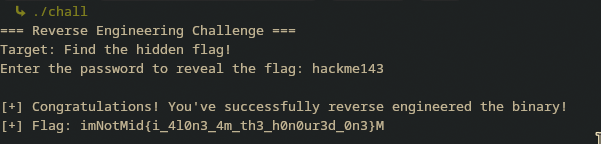
\includegraphics[width=1\linewidth]{figs/jjk4.png}
    \caption{"Throughout Heaven and Earth, I Alone Am The Honored One", Kit-Kat}
    \label{fig:enter-label}
\end{figure}
\end{document}
